\chapter{Modular Approach} \label{ch:modularApproach}
% - what is a modular approach
% - why is it important
%   - extendability
%   - maintainability
%   - reusability
% - all modules in basic form
%   - always imrpoovements possible
% - access != modules to rest
% - both specific to culling as to LDBIM viewers in general
% - knowledge was mined from prototype

This chapter describes a theoretical modular approach for the implementation of this thesis' proposed \ac{ldbim} viewer and associated culling techniques. This design principle consists of separate, independent modules, with each module responsible for a specific functionality of the framework. They are designed to be compatible with any web development framework. The modular approach is important for the following reasons:

\begin{itemize}
  \item \textbf{Extendability}: The modular approach makes it easy to extend the framework with new functionalities, allowing for the addition of new features without altering existing ones.
  \item \textbf{Maintainability}: Modules form meaningful units, making it easy to maintain and update the framework. The structure is easily readable, enabling targeted updates or maintenance efforts.
  \item \textbf{Reusability}: The reusability of modules allows them to be implemented in other projects. This section proposes the role each module should have in the framework, facilitating extrapolation to other web development frameworks.
\end{itemize}

The modules are designed to be specific to both the culling and the \ac{ldbim} viewer. The theoretical model proposed in this thesis is informed by practical experiences and observations gained through the development of the prototype.

The main module, the viewer, and its requirements (Section \ref{sec:viewerRequirements}) have already been discussed in Chapter \ref{ch:dynamicQueries}.

\section{Data fetching}
% - what I mean by that
This section discusses the modules responsible for retrieving external data. Two sub-modules can be identified: the \ac{sparql} fetcher and the database fetcher. The \ac{sparql} fetcher handles communication with the \ac{rdf} database and \ac{sparql} endpoint, while the database fetcher manages communication with external databases where geometry files may be stored. The primary function of these modules, with respect to data fetching, involves authentication and error handling for requests.

Authentication and error handling are crucial when facilitating communication between multiple web instances, such as the website, database, and \ac{sparql} endpoint. By incorporating these functionalities into separate modules, the framework can be adapted to suit the requirements of each use case. This allows for different authentication methods and error handling procedures to be employed, depending on the technology used by each web instance.

\subsection{\acs{sparql} fetcher}
% - handles back and forth communication with rdf database
% - authentication

This module handles the back and forth communication with the \ac{rdf} database and \ac{sparql} endpoint. It should do this on two occasions:

\begin{itemize}
  \item When the \ac{sparql} query is updated, fetching the results of the query from the \ac{sparql} endpoint. This includes the metadata of every given entity provided by the \ac{sparql} endpoint for the cache manager.
  \item When the entities are approved by the cache manager, fetching the geometry literals from the \ac{rdf} database, via the \ac{sparql} endpoint.
\end{itemize}

As mentioned above, the \ac{sparql} fetcher retrieves data from the \ac{sparql} endpoint and is not an endpoint itself. This is done to offload the querying from the viewer, which is a resource-intensive task. It also implies that this module is responsible for the authentication of the connection, error handling, and result interpretation. Metadata about entities is dispatched from this module to the cache manager, waiting for approval before a new query is sent for the retrieval of geometry literals. Once loaded, these literals are dispatched to the viewer for rendering.

Serving two main functions but only communicating with one web instance, the choice was made to combine the two functions into one module. This allows for sharing the same authentication and error handling procedures.

\subsection{Database fetcher}
% - handles back and forth communication with external database
% - authentication
This module, triggered by the cache manager, retrieves the geometry files from an external file server/database. Similar to the \ac{sparql} fetcher, it is responsible for authentication and error handling. It is also responsible for the interpretation of the results, dispatching the geometry files to the viewer for rendering.

\section{Cache manager}
% - what I mean by that
% - why is it important
%   - performance
%   - data integrity
% - multitidude of possibilities, such as LRU
% - why not others

The cache manager is responsible for managing the cache. It is the module that decides which entities are to be cached and which are to be removed from the cache and subsequently from the viewer. This module is crucial for the performance of the framework, as it determines which entities are to be added and which are to be removed from the viewer. It is also responsible for maintaining the integrity of the metadata about entities in the viewer, ensuring that the cache is not filled with outdated metadata.

It therefore evaluates if results from the \ac{sparql} fetcher already exist in the viewer/cache, and if so, whether they are up to date. If the results are not up to date or propose a new entity, the cache manager will trigger the fetching of the new geometry by the appropriate fetcher. The cache manager is also responsible for keeping track of the entities in the viewer and removing them when they are no longer relevant or outdated.

This last functionality requires the use of a cache replacement algorithm. The algorithm determines which entities are to be removed from the viewer, based on a set of rules such as: the number of entities in the viewer, the time since the entity was last viewed, the number of times the entity was viewed, etc. To illustrate the functionality, the following section will discuss the \ac{lru} algorithm. This algorithm was chosen because of its simplicity and ease of implementation. It is also a popular algorithm for cache replacement and is therefore a good starting point for the development of the framework. Some other possible algorithms are, for example, the \ac{lfu}, \ac{fifo}, \ac{lifo}, and \ac{mru} algorithms\parencite{cacheAlgorigthms}. These algorithms are not discussed in this thesis but are possible candidates for future research, as they may be better suited for the framework.

\subsection{\acs{lru} algorithm}
% - LRU principle
% - develop needs
As a possible cache replacement algorithm, the \ac{lru} algorithm limits the number of entities allowed in the viewer. It can be interpreted as a list in which new entities are added at the front of the list, and existing entries are also moved back to the front. The addition of a new entity thus shifts the existing entities back in the list. When an existing entity is viewed again, it moves back to the front of the list without shifting the tail of the list. When the list is full, the entity at the end of the list is removed from the viewer, as it is the least recently used entity \parencite{cacheAlgorigthms}.

To implement this algorithm, the cache manager needs to store the metadata of each new entity, or if the entity already exists, compare the new metadata about it and move it to the front of the list, triggering the fetching modules.

\section{Query processing}
% - multiple sources

The query processing module proposed by this thesis comprises multiple sub-modules aiming to assemble the \ac{sparql} query from different sources, such as the \ac{ui}, culling algorithm, and other user-specific settings.

\subsection{Query builder}
% - challenges that come with it
% - abstraction of dynamic queries in algorithms, 

To facilitate the construction of the \ac{sparql} query, the query builder module is responsible for assembling the query from the different requirements stated by the culling algorithms, thereby constructing a query that complies with the various algorithms in one. It concatenates the abstractions stated by these algorithms into one coherent query, reducing the load on the \ac{sparql} fetcher.

The sub-functions or culling algorithms of this module need access to the rest of the framework. As illustrated in Sections \ref{sec:inSituWKT}, \ref{sec:inViewer}, and \ref{sec:inQuery}, it will require communication with the viewer to retrieve the camera position and execute 3D operations.

\subsection{Query composer}
% - combination af multiple queries

As the \ac{ui} interactions can override the query generated by the building module, the query composer module is responsible for combining the query from the query builder with the query parameters from the \ac{ui}. Performing a final check on the query, it ensures that the query is valid and ready to be sent to the \ac{sparql} fetcher.

By separating this module from the builder, the builder can focus on the construction of the culling query, while the composer can concentrate on the combination of the query with the \ac{ui} parameters apart from the culling query.

\section{Interactions} \label{sec:interactions}
% - diagram + explanations

All the modules come together in one flexible framework illustrated in Figure \ref{fig:interactionModules}. Four main modules create the proposed framework. The query processing module, once fed with data from both the cache manager and viewer, concatenates the different sub-modules to the query composer, creating a \ac{sparql} query. This query creation triggers a first request to the \ac{sparql} endpoint, which returns metadata about the needed entities. Once approved by the cache manager, to avoid constantly reloading the geometry data, it gets dispatched to the \ac{sparql} or database fetcher. The retrieved geometry data is then sent to the viewer for rendering. Afterward, the cycle starts again, feeding viewer and cache manager data to the dynamic culling query algorithms.

\begin{figure}[H]
  \centering
  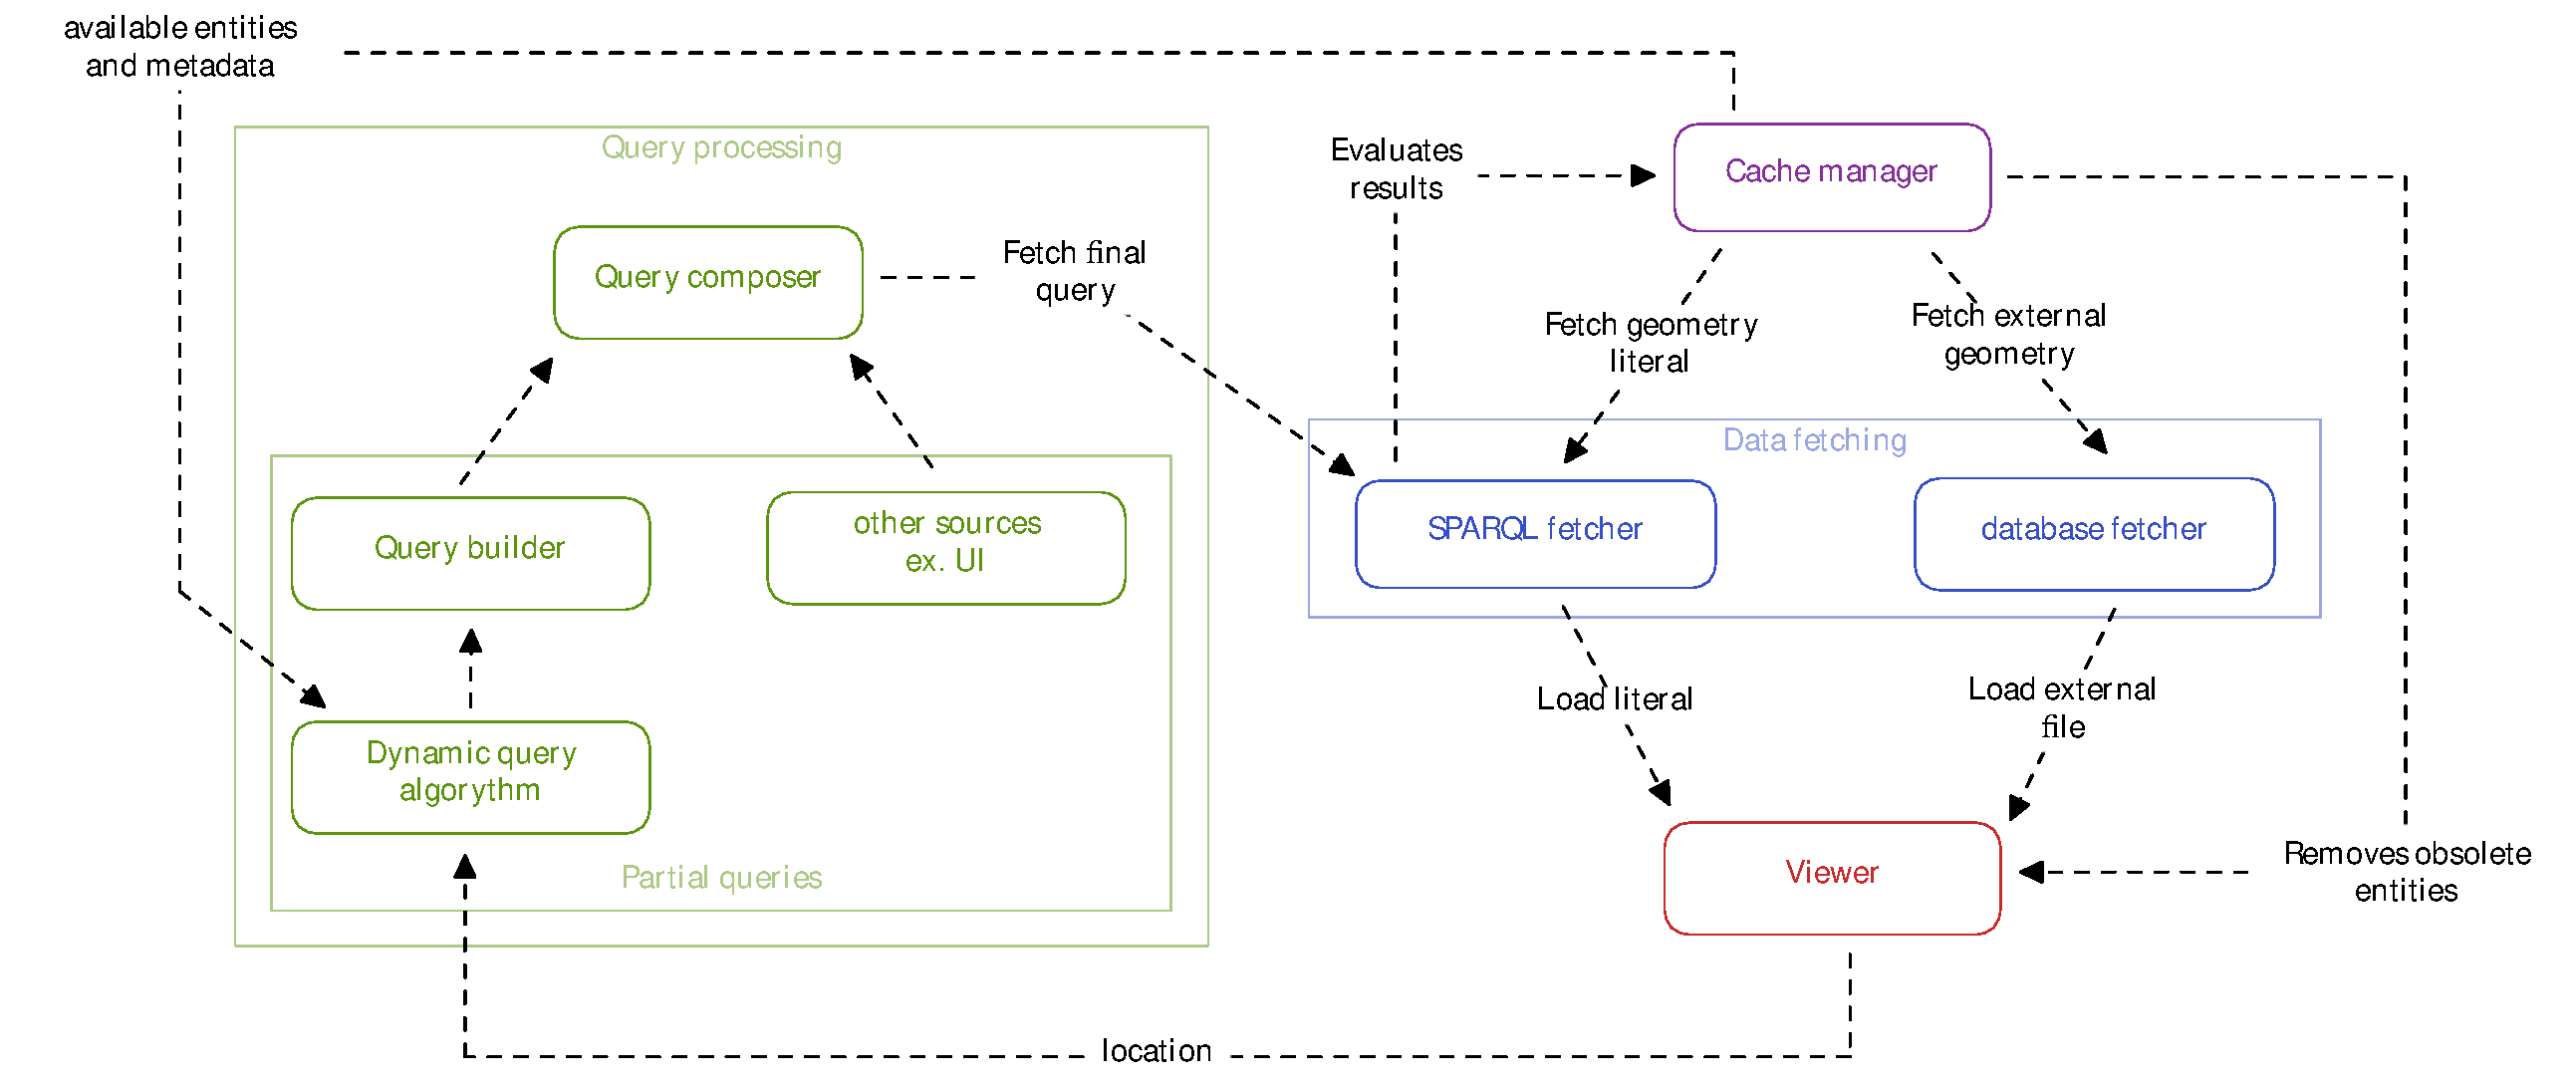
\includegraphics[width=\textwidth]{figures/pdf/interactions_concept.pdf}
  \caption[Interactions modular framework]{Conceptual diagram of the interactions between the modules.}
  \label{fig:interactionModules}
\end{figure}

\section{Sequences}
